\documentclass{beamer}
\usepackage{graphicx} % Required for inserting images
\usepackage{mathtools}
\usepackage[backend=biber]{biblatex}
\usepackage{bookmark}
\usepackage{thmtools}
\graphicspath{ {./photos/} }
\usetheme[progressbar=frametitle]{metropolis}
\usepackage{appendixnumberbeamer}
\usepackage{booktabs}
\usepackage[scale=2]{ccicons}
\usepackage{pgfplots}
\usepgfplotslibrary{dateplot}
\usepackage{xspace}
\usepackage{wrapfig}
\usepackage{url}
\newcommand{\themename}{\textbf{\textsc{metropolis}}\xspace}
\setbeamercolor{block body alerted}{bg=alerted text.fg!10}
\setbeamercolor{block title alerted}{bg=alerted text.fg!20}
\setbeamercolor{block body}{bg=structure!10}
\setbeamercolor{block title}{bg=structure!20}
\setbeamercolor{block body example}{bg=green!10}
\setbeamercolor{block title example}{bg=green!20}
\usepackage[font={tiny,it}]{caption}
\usepackage[export]{adjustbox}
\usepackage{verbatim}
\usepackage{biblatex}
\usepackage{verbatimbox}
\newcommand\scalemath[2]{\scalebox{#1}{\mbox{\ensuremath{\displaystyle #2}}}}

%\captionsetup{justification=raggedleft,singlelinecheck=false}
\title{Row Reduction and Inverse Calculator}
\author{Andrew Ye and James Ross}
\date{May 2024}

\begin{document}
\frame{\titlepage}

\begin{frame}
\frametitle{Table of Contents}
\setbeamertemplate{section in toc}[sections numbered]
\tableofcontents
\end{frame}

\begin{frame}{Objective}
    Our objective for this project was to create a program that would allow the user to perform matrix operations found in a linear algebra class.
\end{frame}

\section{Accessing the Calculator}

\begin{frame}{Github}
    Go to this link \url{https://github.com/AndrewYe12/RREF}. Download the \(alltogether.py\) and \(execute.py\) files. \\
    \begin{center}
    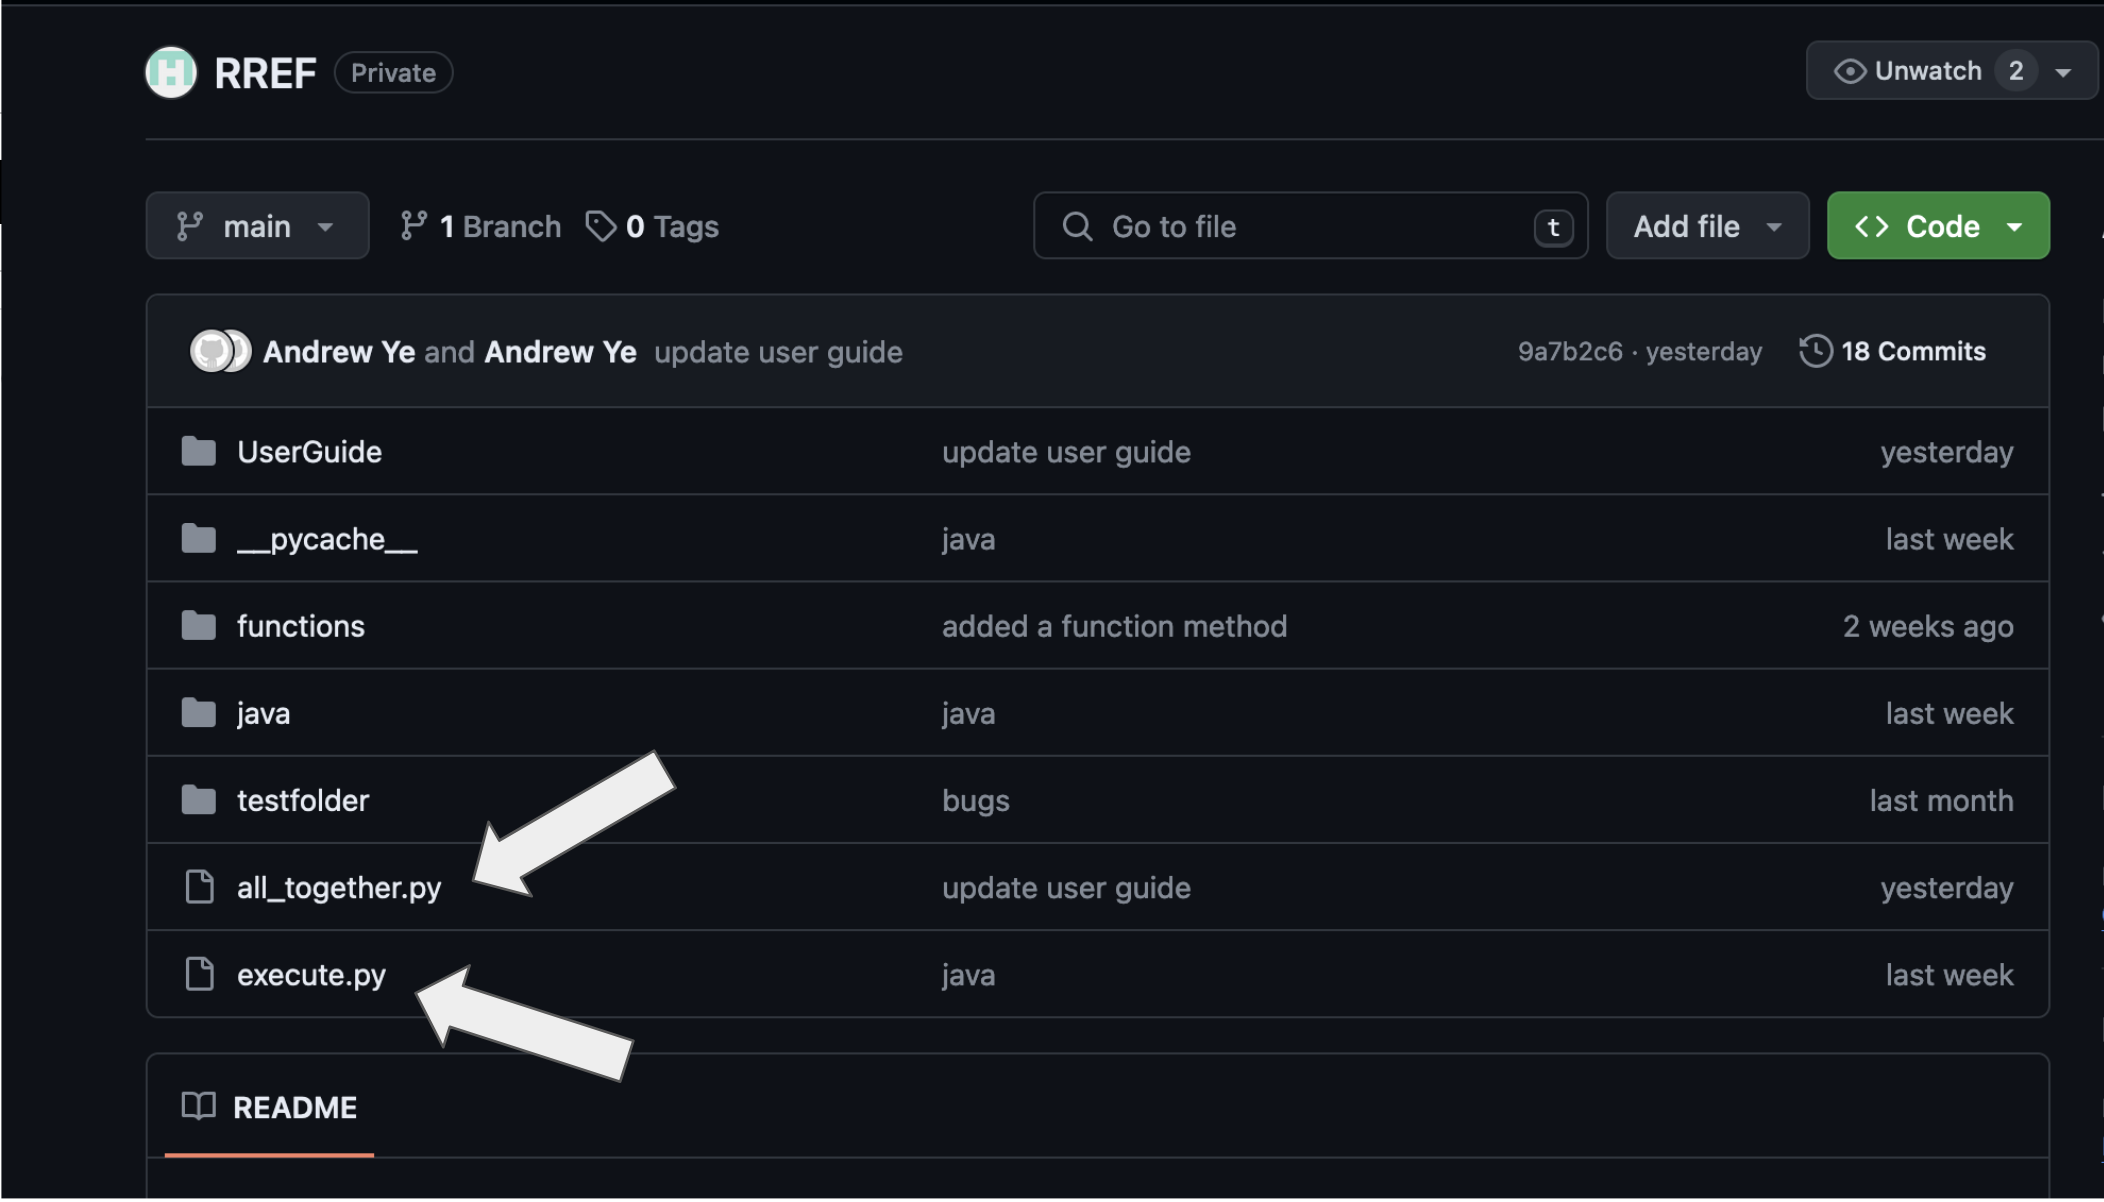
\includegraphics[scale = 0.3]{photos/photo2.png}
    \end{center}
\end{frame}

\section{Using the Calculator}

\begin{frame}[fragile = singleslide]\frametitle{Creating Your Matrix}
    To encode your matrix in a way the program can act upon you must format it as a list of lists of integers, with each list of numbers representing a row.
\begin{verbatim}
x = matrix([[1,2],[2,1]]) 
\end{verbatim}
\begin{equation*}
\left[ \begin{array}{cc} 1&2 \\ 2&1 \end{array}\right]
\end{equation*}
\end{frame}


\section{Matrix Operations as Methods}
\begin{frame}{Our Methods}
We wanted to program an algorithm to row reduce a matrix, find the inverse of a matrix, add/multiply two matrices, and find the determinant of a matrix.
\end{frame}
\begin{frame}{Intro to Matrix Operation Methods}
    \begin{center}
        $.rref()$: Reduces the matrix to reduced echelon form
        
        $.inverse()$: Finds and returns the inverse of the matrix

        $+$ : Adds two matrices together

        $*$ : Multiplies two matrices together

        $.fraction()$: Returns the matrix as a string of fractions

        \(.det()\): Calculates the determinant of a matrix. 
    \end{center}
\end{frame}

\begin{frame}[fragile=singleslide]\frametitle{Row Reduction}
Transforms a matrix into row reduced echelon form.
\begin{verbatim}
from all_together import matrix
x = matrix([[-3,3,4,5], [2,2,3,3],[2,2,3,22]])
print(x.rref().matrix) 
\end{verbatim}
\begin{equation*}
\left[
\begin{array}{cccc}
    -3 & 3 & 4 &5   \\
     2&2&3&3 \\
     2&2&3&22
\end{array}
\right]
\rightarrow
\left[
\begin{array}{cccc}
    1 & 0 & 0.08333333333333326 &0   \\
     0&1& 1.4166666666666665&0 \\
     0&0&0&1
\end{array}
\right]
\end{equation*}
\end{frame}

\begin{frame}[fragile = singleslide]\frametitle{Inverse}
Outputs the inverse of a matrix.
\begin{verbatim}
from all_together import matrix
x = matrix([[-3,3,4,5], [2,2,3,3],[2,2,3,22]])
print(x.inverse().matrix) 
\end{verbatim}
\(A = \left[ \begin{array}{cccc} -3&3&4&5 \\ 2&2&3&3 \\ 2&2&3&22 \end{array}\right]\). This code finds the matrix \\ \(P = \left[ \begin{array}{cccc} -0.166666666&0.24561403&0.00438596491 \\ 0.16666666666&0.333333333&-0.08333333 \\ 0&-0.0526315789&0.0526315789 \end{array}\right]\) so that 
\begin{equation*}
     PA = rref(A) 
\end{equation*}
\end{frame}

\begin{frame}[fragile = singleslide]{Addition}
Inputs two matrices and returns one with the added terms.
\begin{verbatim}
from all_together import matrix
x = matrix([[-3,3,4,5], [2,2,3,3],[2,2,3,22]])
y = matrix([[-3,3,4,10], [2,22,3,3],[2,11,3,22]])
print((x + y).matrix) 
\end{verbatim}
\begin{equation*}
    \left[
    \begin{array}{cccc}
    -3 & 3 & 4 &5   \\
     2&2&3&3 \\
     2&2&3&22
    \end{array}
    \right]
    +
    \left[
    \begin{array}{cccc}
    -3 & 3 & 4 &10   \\
     2&22&3&3 \\
     2&11&3&22
    \end{array}
    \right]
    =
    \left[
    \begin{array}{cccc}
        -6 & 6&8&15 \\
        4 &24&6&6\\
        4&13&6&44
    \end{array}
    \right]
\end{equation*}
\end{frame}

\begin{frame}[fragile = singleslide]{Multiplication}
Inputs two matrices and outputs the matrix resulting from performing matrix multiplication.
\begin{verbnobox}[\fontsize{8pt}{8pt}\selectfont]
from all_together import matrix
x = matrix([[-3,3,4,5], [2,2,3,3],[2,2,3,22]])
y = matrix([[-3,3,4,10,9], [2,22,3,3,8],[2,11,3,22,7],[4,2,1,34,5]])
print((x * y).matrix) 
\end{verbnobox}
\begin{equation*}
\scalebox{0.8}{$
\left[
    \begin{array}{cccc}
        -3 &3&4&5  \\
         2&2&3&3\\
         2&2&3&22
    \end{array}
\right]
    \left[
    \begin{array}{ccccc}
        -3 &3&4&10&9  \\
         2&22&3&3&8\\
         2&11&3&22&7\\
         4&2&1&34&5
    \end{array}
    \right] 
    =
    \left[
    \begin{array}{ccccc}
        43 &111&14&237&50  \\
         16&89&26&194&70\\
         92&127&45&840&165
    \end{array}
    \right]
$}
\end{equation*}



\end{frame}

\begin{frame}[fragile = singleslide]{Fraction}
Inputs a matrix and returns a copy of it with the entries as fractions.
\begin{verbatim}
from all_together import matrix    
x = matrix([[-3,3,4,5], [2,2,3,3],[2,2,3,22]])
print(x.fraction().matrix) 
\end{verbatim}
\begin{equation*}
    \left[ \begin{array}{cccc} -3&3&4&5 \\ 2&2&3&3 \\ 2&2&3&22 \end{array}\right]
    \rightarrow
    \left[
    \begin{array}{cccc}
        \text{`}\frac{-3}{1}\text{'} &\text{`}\frac{3}{1}\text{'}&\text{`}\frac{4}{1}\text{'}&\text{`}\frac{5}{1}\text{'}  \\
         \text{`}\frac{2}{1}\text{'}&\text{`}\frac{2}{1}\text{'}&\text{`}\frac{3}{1}\text{'}&\text{`}\frac{3}{1}\text{'}\\
         \text{`}\frac{2}{1}\text{'}&\text{`}\frac{2}{1}\text{'}&\text{`}\frac{3}{1}\text{'}&\text{`}\frac{22}{1}\text{'}
    \end{array}
    \right]
\end{equation*}

\end{frame}

\begin{frame}[fragile = singleslide]{Determinant}
    Inputs a matrix and returns the determinant. 
\begin{verbatim}
from all_together import matrix    
x = [[1,0,0],[0,1,0],[0,0,1]]
print(x.det()) 
\end{verbatim}
\begin{equation*}
    det \left[
    \begin{array}{ccc}
        1 & 0 &0 \\
        0 &1&0 \\
        0&0&1 
    \end{array}
    \right] = 1
\end{equation*}
\end{frame}


\section{Reflection}
\begin{frame}{What Went Well}
    The matrix multiplication and addition methods were relatively easy to implement because they had an explicit formula. For example, if \(A\) is a \(m \times n\) matrix and \(B\) is a \(n \times p\) matrix, then
    \begin{equation}
        (AB)_{ij} = \sum^{n}_{r=1}A_{ir}*B_{rj}
    \end{equation}
\end{frame}

\begin{frame}{Problems We Faced}
    The inverse and row reduction methods were difficult to implement. The hardest part was swapping the rows. The rows only have a position relative to each other. 
    \begin{equation*}
    \left[
        \begin{array}{cccc}
            0 & 1&0&0  \\
            0 & 0&0&1 \\
            1&0&0&0
        \end{array}
    \right]
    \rightarrow
    \left[
    \begin{array}{cccc}
        1 &0&0&0  \\
         0&1&0&0\\
         0&0&0&1
    \end{array}
    \right]
    \end{equation*}
\end{frame}

\begin{frame}{Results}
    This program has already helped us in our linear algebra class by allowing us to compute these steps in an efficient way. \pause
\begin{center}
    Are there any questions?
\end{center}

\end{frame}



\end{document}
